\documentclass{article}
\usepackage{amsmath}
\usepackage{amssymb}
\usepackage{bm}
\usepackage{graphicx}
\usepackage{epstopdf}
\DeclareGraphicsRule{.tif}{png}{.png}{`convert #1 `basename #1 .tif`.png}
\usepackage{color}
\pagestyle{plain}
%\pagestyle{empty}
\textheight 9 true in
\textwidth 6.5 true in
\hoffset -.75 true in
\voffset -.75 true in
 
\mathsurround=2pt  \parskip=2pt
\def\crv{\cr\noalign{\vskip7pt}} 
\def\a{\alpha } \def\b{\beta } \def\d{\delta } \def\D{\Delta } \def\e{\epsilon }
\def\g{\gamma } \def\G{\Gamma} \def\k{\kappa} \def\l{\lambda } \def\L{\Lambda }
\def\th{\theta } \def\Th{\Theta} \def\r{\rho} \def\o{\omega} \def\O{\Omega}
\def\ve{\varepsilon} 

\def\sA{{\cal A}} \def\sB{{\cal B}} \def\sC{{\cal C}} \def\sI{{\cal I}}
\def\sR{{\cal R}} \def\sF{{\cal F}} \def\sG{{\cal G}} \def\sM{{\cal M}}
\def\sT{{\cal T}} \def\sH{{\cal H}} \def\sD{{\cal D}} \def\sW{{\cal W}}
\def\sL{{\cal L}} \def\sP{{\cal P}} \def\s{\sigma } \def\S{\Sigma}
\def\sU{{\cal U}} \def\sV{{\cal V}} \def\sY{{\cal Y}}

\def\gm{\gamma -1}
\def\summ{\sum_{j=1}^4}

\def\bb{{\bm b}} \def\yb{{\bm y}}
\def\ub{{\bm u}}  \def\xb{{\bm x}} \def\vb{{\bm v}} \def\wb{{\bm w}}
\def\omegab{{\bm \omega}} \def\rb{{\bm r}} \def\ib{{\bm i}} \def\jb{{\bm j}}
\def\lb{{\bm l}} \def\kb{{\bm k}} \def\Ab{{\bm A}} \def\fb{{\bm f}} \def\Ub{{\bm U}}
\def\Fb{{\bm F}} \def\nb{{\bm n}} \def\Db{{\bm D}} \def\eb{{\bm e}}
\def\gb{{\bm g}}  \def\Gb{{\bm G}} \def\hb{{\bm h}} \def\Yb{{\bm Y}} \def\Rb{{\bm R}} 
\def\Tb{{\bm T}}

\def\As1{{\bf {\cal A}}_1}\def\DO{{\cal D}_0} \def\UO{{\cal U}_0}
\def\ie{{\it{i.e.}}}

\def\ubbar{{\bf {\bar{u}}}} \def\sbar{{\bar{\sigma }}} \def\ubar{{\bar{u}}}  
\def\abar{{\bar{a}}} \def\vbar{{\bar{v}}}  \def\rbar{{\bar{\rho}}}
\def\pbar{{\bar{p}}} \def\ebar{{\bar{e}}} \def\Tbar{{\bar{T}}}
\def\bbar{{\bar{\beta}}} \def\Mbar{{\bar{M}}}  \def \sMbar{{\bar{\cal M}}}
\def\Ebar{{\bar{E}}} \def\sMbar{{\bar{\cal M}}}
\def\sPbar{{\bar{\cal P}}} \def\xbar{{\bar{x}}}

\newcommand{\pdv}[2]{\frac{\partial#1}{\partial#2}}
\newcommand{\dv}[2]{\frac{d#1}{d#2}}
\newcommand{\ord}[2]{#1^{(#2)}}
\newcommand{\vct}[1]{\vec{#1}}

 \newcommand{\bc}{\begin{center}}
 \newcommand{\ec}{\end{center}}
 
 \newcommand{\bq}{\begin{equation}}
 \newcommand{\eq}{\end{equation}}
 
 \newcommand{\beqs}{\begin{eqnarray}}
 \newcommand{\eeqs}{\end{eqnarray}}
 
 \newcommand{\beqa}{\begin{eqnarray*}}
 \newcommand{\eeqa}{\end{eqnarray*}}
 
 \newcommand{\ol}{\overline}
 \newcommand{\ul}{\underline}
 
 \newcommand{\dint}{{\int \!\! \int \!\!}}
 \newcommand{\tint}{{\int \!\! \int \!\! \int \!\!}}
 
 \newcommand{\bfig}{\begin{figure}}
 \newcommand{\efig}{\end{figure}}
 
 \newcommand{\cen}{\centering}
 \newcommand{\n}{\noindent}
 
 \newcommand{\btab}{\begin{table}}
 \newcommand{\etab}{\end{table}}
 
 \newcommand{\btbl}{\begin{tabular}}
 \newcommand{\etbl}{\end{tabular}}
 
 \newcommand{\bdes}{\begin{description}}
 \newcommand{\edes}{\end{description}}
 
 \newcommand{\benum}{\begin{enumerate}}
 \newcommand{\eenum}{\end{enumerate}}
 
 \newcommand{\bite}{\begin{itemize}}
 \newcommand{\eite}{\end{itemize}}
 
 \newcommand{\cle}{\clearpage}
 \newcommand{\npg}{\newpage}
 
 \newcommand{\bss}{\begin{singlespace}}
 \newcommand{\ess}{\end{singlespace}}
 
 \newcommand{\bhalf}{\begin{onehalfspace}}
 \newcommand{\ehalf}{\end{onehalfspace}}
 
 \newcommand{\bds}{\begin{doublespace}}
 \newcommand{\eds}{\end{doublespace}}
 
 \newcommand{\eps}{\mbox{$\epsilon$}} 
 \newcommand{\stilde}{\mbox{$\tilde s$}} 
 \newcommand{\shat}{\mbox{$\hat s$}} 

 \newcommand{\blue}{\color{blue}}
 \newcommand{\red}{\color{red}}
 \newcommand{\magenta}{\color{magenta}}
 \newcommand{\green}{\color{green}}
 \newcommand{\nc}{\normalcolor}





\newcommand{\Ai}{{\rm Ai}}
\newcommand{\Bi}{{\rm Bi}}
\pagestyle{empty}
\begin{document}

\begin{center}
\large{ MATH-6620 \hspace{1in}  PERTURBATION METHODS \hspace{1in}SPRING 2016\\ Final Examination \\ Due Wednesday May 18, by 5:00 PM. }\end{center}

\bigskip
\n\ul{Michael Hennessey}\\
{\bf I have abided by the ground rules of this examination}

\bc {\bf PROBLEMS} \ec

\benum
\item Find the asymptotic expansions, as $x\to\infty$, of the solutions of the ODE
$$y''+x^2y'+xy=0.$$
Solution:\\

We begin by making the transformation
$$y(x)=z(x)Exp[-\frac{1}{2}\int x^2dx]=z(x)e^{-x^3/6}.$$
This results in the ODE
$$z''-\frac{x^4}{4}z=0.$$
We now let $z=e^{\phi(x)}$ and find
$$\phi''+\phi'^2-\frac{x^4}{4}=0.$$
Since $x^4/4$ is of the form $x^\alpha$, and since $\alpha=4>-2$, we suspect dominant balance lies between the terms $\phi'^2$ and $x^4/4$. Setting these equal to one another results in
$$\phi_0=\pm \frac{x^3}{6}.$$
Thus we have the first term of each solution. Now, we split our solution up into two cases.
\benum
\item Case 1: $\phi_0=x^3/6.$ We determine the next term in $\phi$ by setting $\phi\sim x^3/6+\phi_1.$ Substituting this into the ODE for $\phi$ gives
    $$ (x+\phi_1'')+(\frac{x^4}{4}+x^2\phi_1'+\phi_1'^2)-\frac{x^4}{4}=0.$$
    After performing the obvious cancellation, we argue that balance holds in this equation from the remaining first terms in the parentheses.
    $$x+x^2\phi_1'\sim 0\;\implies\;\phi_1\sim -\ln x.$$
    If we continue on to the next term, by setting $\phi\sim x^3/6-\ln x+\phi_2$, we get the ODE
    $$(x+\frac{1}{x^2}+\phi_2'')+(\frac{x^4}{4}-x+\frac{2}{x^2}+x^2\phi_2'-\frac{2\phi_2'}{x}+\phi_2'^2)-\frac{x^4}{4}=0.$$
    After going trough the same process as before, we have
    $$\frac{3}{x^2}+x^2\phi_2'\sim 0\;\implies\; \phi_2\sim\frac{1}{x^3}.$$
    Thus first asymptotic expansion is
    $$y\sim \frac{1}{x}e^{1/x^3}\sim \frac{1}{x}[1+\frac{1}{x^3}+\frac{1}{2x^6}].$$

\item Case 2: $\phi_0=-x^3/6.$ We now follow the same procedure as above. $\phi\sim -x^3/6+\phi_1.$ The ODE is then
$$(-x+\phi_1'')+(\frac{x^4}{4}-x^2\phi_1'+\phi_1'^2)-\frac{x^4}{4}=0.$$
$$\implies -x-x^2\phi_1'=0\;\implies\; \phi_1=-\ln x.$$
Next, $\phi\sim -x^3/6-\ln x+\phi_2.$ Now the ODE becomes
$$(-x+\frac{1}{x^2}+\phi_2'')+(\frac{x^4}{4}+x+\frac{1}{x^2}-x^2\phi_2'-\frac{2\phi_2'}{x}+\phi_2'^2)-\frac{x^4}{4}=0.$$
$$\implies\; \frac{2}{x^2}-x^2\phi_2'=0\;\implies \; \phi_2=-\frac{2}{3x^3}.$$
Thus our second asymptotic expansion is
$$y\sim \frac{1}{x}e^{-x^3/3}[1-\frac{2}{3x^3}+\frac{2}{9x^6}].$$

\eenum
\item Find the first few terms in the asymptotic expansion, as $\lambda\to\infty$, of the solutions of
    $$y''+\left(\frac{\lambda^2}{x}+1\right)y=0,\;\;|x|>0.$$
    Solution:\\

    Although the function multiplying $\lambda^2$ changes sign at $x=0$, it never passes through 0, and is thus not a typical turning point. Furthermore,  as $x=0$ is excluded from the domain of the problem, we may simply ignore the singularity of the problem at this point. We will discuss this further once the solution has been determined. We begin, then, by letting
    $$y(x)=e^{\lambda\o(x)}\phi(x)\left[1+\frac{1}{\lambda}f_1(x)+\frac{1}{\lambda^2}f_2(x)\right].$$
    When we substitute this into our ODE and group by powers of $\lambda$, we find
    $$\lambda^2 \left[\o'^2\phi+\frac{\phi}{x}\right]+\lambda\left[\o''\phi+\o'^2\phi f_1+2\o'\phi'+\frac{\phi f_1}{x}\right]+\left[\o''\phi f_1+\o'^2\phi f_2+2\o'\phi'f_1+2\o'\phi f_1'+\phi''+\frac{f_2\phi}{x}+\phi\right]=0.$$
    If we then treat each coefficient of the powers of $\lambda$ as separate equations, we see
    $$\o'^2\phi+\frac{\phi}{x}=0\;\implies \;\o=\pm i2\sqrt{x}.$$
    $$\o''\phi+2\o'\phi'=0\;\implies \; \phi=x^{1/4}.$$
    $$2\o'\phi f_1'+\phi''+\phi=0\;\implies\; f_1=\pm\frac{3 i}{32 x}\pm\frac{ix^{3/2}}{3}.$$
    Fortunately, this actually results in two solutions, as the $\pm$ signs for $f_1$ and $\o$ are connected. Thus we have
    $$y\sim e^{2\lambda i\sqrt{x}}x^{1/4}\left[1+\frac{3i}{32x}+\frac{i x^{3/2}}{3}\right]$$
    and
    $$y\sim e^{-2\lambda i\sqrt{x}}x^{1/4}\left[1-\frac{3i}{32 x}-\frac{ix^{3/2}}{3}\right].$$
    Now we see that there is no issue for $|x|>0$ for either solution, and thus our problem does not have a turning point.

\item Consider the fourth-order ODE
$$\e^2y^{iv}-\frac{1}{1-(3x/4)}y''=8,\;\;0<x<1,$$
with boundary conditions
$$y(0)=y'(0)=y(1)=y'(1)=0.$$
\benum
\item Anticipating boundary layers at both ends, find a one-term outer solution.
\item Find each boundary-layer solution to one term, keeping in mind that the dependent variable may not be order unity there.
\eenum

Solution:\\

\benum \item To determine the outer solution, we let $y(x;\e)\sim y_0(x)$ and find
$$-\frac{4}{4-3x}y_0''=8.$$
Thus the outer solution is
$$y_0=x^3-4x^2+c_1 x+c_2.$$
The constants $c_1$ and $c_2$ will be determined from matching.
\item Now we determine the boundary-layer solution at $x=0.$ We let $\delta \xi=x$, and $y(x;\e)=u(\xi;\e)$ to find
    $$\frac{\e^2}{\delta^4}u^{iv}-\frac{4}{(4-3\delta \xi)\delta^2}u''=8.$$
    Dominant balance requires
    $$\frac{\e^2}{\delta^4}=\frac{1}{\delta^2}\;\implies\;\delta=\e.$$
    Thus our ODE is
    $$u^{iv}-\frac{4}{4-3\e\xi}u''=8\e^2.$$
    We let $u(\xi;\e)\sim u_0(\xi)$ and find
    $$u_0^{iv}-u_0''=0.$$
    Thus the solution in this layer is
    $$u_0=b_1e^{\xi}+b_2e^{-\xi}+b_3\xi+b_4.$$
    Applying the boundary conditions at $x=0$ gives
    $$u_0=b_1\left(e^{\xi}-\xi-1\right)+b_2\left(e^{-\xi}+\xi-1\right).$$
    The coefficients $b_1$ and $b_2$ will be determined from matching.\\
    \indent We next find the boundary-layer solution at $x=1.$ We let $\delta\eta=x-1,$ and $y(x;\e)=v(\eta;\e.$ This gives us the ODE
    $$\frac{\e^2}{\delta^4}(1-3\delta\eta)-\frac{4}{\delta^2}v''=8(1-3\delta\eta),$$
    with initial conditions $v(0)=v'(0)=0.$ Dominant balance will again require that $\e=\delta.$ Thus we let $v(\eta;\e)\sim v_0(\eta)$ and solve
    $$v_0^{iv}-4v_0''=0.$$
    $$v_0=\frac{B_1}{4}e^{2\eta}+\frac{B_2}{4}e^{-2\eta}+B_3\eta+B_4.$$
    Applying the initial conditions gives
    $$v_0=\frac{B_1}{4}(e^{2\eta}-2\eta-1)+B_2(e^{-2\eta}+2\eta-1).$$
    \item Now we attempt to match the inner and outer solutions to find the values of $c_1,c_2,b_1,b_2,B_1,$ and $B_2.$ We begin by arguing that exponential growth in the inner layers is unreasonable, and thus $B_2=b_1=0.$ Now we express $u_0$ and $v_0$ in terms of $x$:
        $$u_0=b_2\left[e^{-x/\e}-1+\frac{x}{\e}\right].$$
        $$v_0=\frac{B_1}{4}\left[e^{-2(1-x)/\e}-1+2\frac{1-x}{\e}\right].$$
        Here we see that matching with the $O(1)$ outer solution will be impossible, since the inner solutions are both $O(1/\e).$ We then must stretch our dependant variable in the inner layers as well. Fortunately, this results in the exact same inner-layer ODEs when we let $y(x;\e)=\e u(\xi;\e)$ and $y(x;\e)=\e v(\eta;\e).$ Therefore, we want to match 
        $$\e u_0=b_2\left[\e(e^{-x/\e}-1)+x\right],$$
        $$\e v_0=\frac{B_1}{4}\left[\e(e^{-2(1-x)/\e}-1)+2-2x\right].$$
        We perform this matching by introducing the intermediate variable $x=\mu(\e)\zeta.$ Then expressing the outer and inner solutions in $\zeta$ gives
        $$y_0=\mu^3\zeta^3-4\mu^2\zeta^2+c_1\mu\zeta+c_2,$$
        $$\e u_0=b_2\left[\e(e^{-\mu\zeta/\e}-1)+\mu\zeta\right],$$
        $$\e v_0=\frac{B_1}{4}\left[\e(e^{-2(1-\mu\zeta)/\e}-1)+2-2\mu\zeta\right].$$
        We then enforce that $y_0-\e u_0=o(1)$ and $y_0-\e v_0=o(1).$ This results in $c_2=0$ and
         $$c_1=\left\{\begin{array}{cc}b_2,&0<x<x_0\\ \frac{1}{2}B_1,&x_0<x<1\end{array}\right.$$
         for some $x_0.$
       Therefore, we must use properties of the equation and the solution to determine the values of $b_2,$ $B_1$, and $x_0$. If we write the additive composite, we find something close to the exact solution, but a better composite is of the form:
       $$y_c=\left\{\begin{array}{cc}x^3-4x^2+b_2 x+\e b_2(e^{-x/\e}-1),&0<x<x_0\\ x^3-4x^2+\frac{B_1}{2}x+\e\frac{B}{4}(e^{-2(1-x)/\e}-1),&x_0<x<1\end{array}\right. .$$
       Using the fact that we want $y_c(0)=y_c(1)=0,$ we find that $B_1=6$. Then, connecting the two together in the middle will require 
       $$b_2x_0+\e b_2(e^{-x_0/\e}-1)=3x_0+\e \frac{3}{2}(e^{-2(1-x_0)/\e}-1).$$
       We then have $b_2$ in terms of $x_0:$
       $$b_2=\frac{3x_0+\frac{3\e}{2}\left(e^{-2(1-x_0)/\e}-1\right)}{x_0+\e(e^{-x_0/\e}-1)}.$$
        Any reasonable choice of $x_0$ in $[.6,.8]$ will give a good approximation of the exact solution.
        A graph of the approximate solution and a graph of the exact solution can be seen below.
        
\begin{figure}
  \centering
  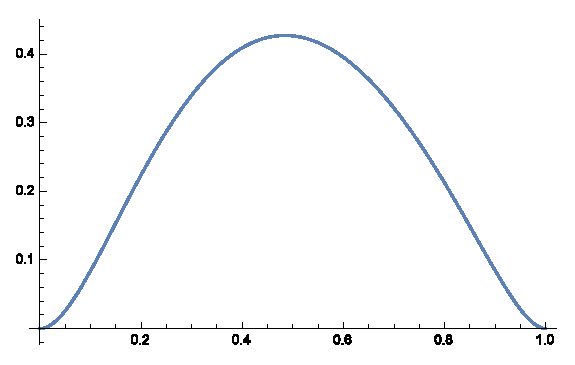
\includegraphics[width=3in]{exactsoln}
  \caption{Numerical solution of exact equation with $\e=.1$}
\end{figure}
\begin{figure}
  \centering
  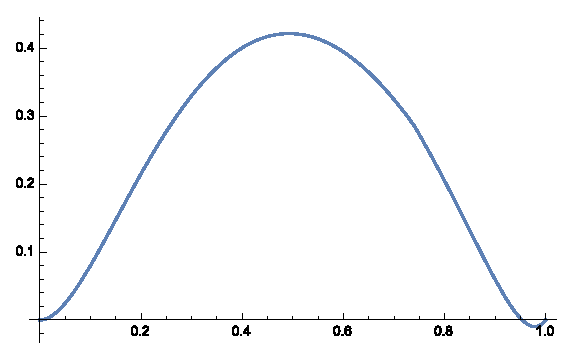
\includegraphics[width=3in]{composite}
  \caption{Composite solution with $x_0=.74$, $\e=.1$.}
\end{figure}

        


        \eenum
        \eenum
        \end{document}
